\documentclass[journal,12pt,twocolumn]{IEEEtran}
\makeatletter
\@addtoreset{figure}{problem}
\makeatother
\usepackage{setspace}
\usepackage{gensymb}
\usepackage{xcolor}
\usepackage{caption}
%\usepackage{multirow}
%\usepackage{multicolumn}
%\usepackage{subcaption}
%\doublespacing
\usepackage{amsmath}
\singlespacing
\usepackage{amsmath}
\usepackage{multicol}
\usepackage{enumerate}	
\usepackage{amssymb}
%\usepackage{iithtlc}
%\usepackage{graphicx}
\usepackage{newfloat}
%\usepackage{syntax}
\usepackage{listings}
\usepackage{color}
%\usepackage{tikz}
\usepackage{tikz}
\usepackage{tkz-euclide}
\usetkzobj{all}

\usepackage[american]{circuitikz}
\usetikzlibrary{shapes,arrows}



%\usepackage{graphicx}
%\usepackage{amssymb}
%\usepackage{relsize}
%\usepackage[cmex10]{amsmath}
%\usepackage{mathtools}
%\usepackage{amsthm}
%\interdisplaylinepenalty=2500
%\savesymbol{iint}
%\usepackage{txfonts}
%\restoresymbol{TXF}{iint}
%\usepackage{wasysym}
\usepackage{amsthm}
\usepackage{mathrsfs}
\usepackage{txfonts}
\usepackage{stfloats}
\usepackage{cite}
\usepackage{cases}
\usepackage{mathtools}
\usepackage{caption}
\usepackage{enumerate}	
\usepackage{enumitem}
\usepackage{amsmath}
%\usepackage{xtab}
\usepackage{longtable}
\usepackage{multirow}
%\usepackage{algorithm}
%\usepackage{algpseudocode}
\usepackage{enumitem}
\usepackage{mathtools}

%\usepackage[framemethod=tikz]{mdframed}
\usepackage{listings}
\usepackage{listings}
    %\usepackage[latin1]{inputenc}                                 %%
    \usepackage{color}                                            %%
    \usepackage{array}                                            %%
    \usepackage{longtable}                                        %%
    \usepackage{calc}                                             %%
    \usepackage{multirow}                                         %%
    \usepackage{hhline}                                           %%
    \usepackage{ifthen}                                           %%
  %optionally (for landscape tables embedded in another document): %%
    \usepackage{lscape}     



%\usepackage{stmaryrd}


%\usepackage{wasysym}
%\newcounter{MYtempeqncnt}
\DeclareMathOperator*{\Res}{Res}
%\renewcommand{\baselinestretch}{2}
\renewcommand\thesection{\arabic{section}}
\renewcommand\thesubsection{\thesection.\arabic{subsection}}
\renewcommand\thesubsubsection{\thesubsection.\arabic{subsubsection}}

\renewcommand\thesectiondis{\arabic{section}}
\renewcommand\thesubsectiondis{\thesectiondis.\arabic{subsection}}
\renewcommand\thesubsubsectiondis{\thesubsectiondis.\arabic{subsubsection}}

% correct bad hyphenation here
\hyphenation{op-tical net-works semi-conduc-tor}

%\lstset{
%language=C,
%frame=single, 
%breaklines=true
%}

%\lstset{
	%%basicstyle=\small\ttfamily\bfseries,
	%%numberstyle=\small\ttfamily,
	%language=Octave,
	%backgroundcolor=\color{white},
	%%frame=single,
	%%keywordstyle=\bfseries,
	%%breaklines=true,
	%%showstringspaces=false,
	%%xleftmargin=-10mm,
	%%aboveskip=-1mm,
	%%belowskip=0mm
%}

%\surroundwithmdframed[width=\columnwidth]{lstlisting}
\def\inputGnumericTable{}                                 %%
\lstset{
language=C,
frame=single, 
breaklines=true
}
 

\begin{document}
%
\tikzstyle{block} = [rectangle, draw,
    text width=4em, text centered, minimum height=3em]
\tikzstyle{sum} = [draw, circle, node distance=3cm]
\tikzstyle{input} = [coordinate]
\tikzstyle{output} = [coordinate]
\tikzstyle{pinstyle} = [pin edge={to-,thin,black}]

\theoremstyle{definition}
\newtheorem{theorem}{Theorem}[section]
\newtheorem{problem}{Problem}
\newtheorem{proposition}{Proposition}[section]
\newtheorem{lemma}{Lemma}[section]
\newtheorem{corollary}[theorem]{Corollary}
\newtheorem{example}{Example}[section]
\newtheorem{definition}{Definition}[section]
%\newtheorem{algorithm}{Algorithm}[section]
%\newtheorem{cor}{Corollary}
\newcommand{\BEQA}{\begin{eqnarray}}
\newcommand{\EEQA}{\end{eqnarray}}
\newcommand{\define}{\stackrel{\triangle}{=}}

\bibliographystyle{IEEEtran}
%\bibliographystyle{ieeetr}

\providecommand{\nCr}[2]{\,^{#1}C_{#2}} % nCr
\providecommand{\nPr}[2]{\,^{#1}P_{#2}} % nPr
\providecommand{\mbf}{\mathbf}
\providecommand{\pr}[1]{\ensuremath{\Pr\left(#1\right)}}
\providecommand{\qfunc}[1]{\ensuremath{Q\left(#1\right)}}
\providecommand{\sbrak}[1]{\ensuremath{{}\left[#1\right]}}
\providecommand{\lsbrak}[1]{\ensuremath{{}\left[#1\right.}}
\providecommand{\rsbrak}[1]{\ensuremath{{}\left.#1\right]}}
\providecommand{\brak}[1]{\ensuremath{\left(#1\right)}}
\providecommand{\lbrak}[1]{\ensuremath{\left(#1\right.}}
\providecommand{\rbrak}[1]{\ensuremath{\left.#1\right)}}
\providecommand{\cbrak}[1]{\ensuremath{\left\{#1\right\}}}
\providecommand{\lcbrak}[1]{\ensuremath{\left\{#1\right.}}
\providecommand{\rcbrak}[1]{\ensuremath{\left.#1\right\}}}
\theoremstyle{remark}
\newtheorem{rem}{Remark}
\newcommand{\sgn}{\mathop{\mathrm{sgn}}}
\providecommand{\abs}[1]{\left\vert#1\right\vert}
\providecommand{\res}[1]{\Res\displaylimits_{#1}} 
\providecommand{\norm}[1]{\lVert#1\rVert}
\providecommand{\mtx}[1]{\mathbf{#1}}
\providecommand{\mean}[1]{E\left[ #1 \right]}
\providecommand{\fourier}{\overset{\mathcal{F}}{ \rightleftharpoons}}
%\providecommand{\hilbert}{\overset{\mathcal{H}}{ \rightleftharpoons}}
\providecommand{\system}{\overset{\mathcal{H}}{ \longleftrightarrow}}
	%\newcommand{\solution}[2]{\textbf{Solution:}{#1}}
\newcommand{\solution}{\noindent \textbf{Solution: }}
\providecommand{\dec}[2]{\ensuremath{\overset{#1}{\underset{#2}{\gtrless}}}}
\DeclarePairedDelimiter{\ceil}{\lceil}{\rceil}
%\numberwithin{equation}{subsection}
\numberwithin{equation}{problem}
%\numberwithin{problem}{subsection}
%\numberwithin{definition}{subsection}
%\makeatletter
%\@addtoreset{figure}{problem}
%\makeatother

%\let\StandardTheFigure\thefigure
%\renewcommand{\thefigure}{\theproblem.\arabic{figure}}
%\renewcommand{\thefigure}{\theproblem}


%\numberwithin{figure}{section}

%\numberwithin{equation}{subsection}
%\numberwithin{equation}{section}
\numberwithin{equation}{problem}
%\numberwithin{problem}{subsection}
\numberwithin{problem}{section}
%%\numberwithin{definition}{subsection}
%\makeatletter
%\@addtoreset{figure}{problem}
%\makeatother
%\makeatletter
%\@addtoreset{table}{problem}
%\makeatother

%\let\StandardTheFigure\thefigure
%\let\StandardTheTable\thetable
%\numberwithin{table}{section}
%%\renewcommand{\thefigure}{\theproblem.\arabic{figure}}
%\renewcommand{\thefigure}{\theproblem}

%%\numberwithin{figure}{section}

%%\numberwithin{figure}{subsection}



\def\putbox#1#2#3{\makebox[0in][l]{\makebox[#1][l]{}\raisebox{\baselineskip}[0in][0in]{\raisebox{#2}[0in][0in]{#3}}}}
     \def\rightbox#1{\makebox[0in][r]{#1}}
     \def\centbox#1{\makebox[0in]{#1}}
     \def\topbox#1{\raisebox{-\baselineskip}[0in][0in]{#1}}
     \def\midbox#1{\raisebox{-0.5\baselineskip}[0in][0in]{#1}}

\vspace{3cm}

\title{ 
	%\logo{
Half Bridge Controlled Rectifier using SCR and Arduino
	%}
}

\author{Supriya Mane and  G V V Sharma$^{*}$% <-this % stops a space
	\thanks{*The author is with the Department
		of Electrical Engineering, Indian Institute of Technology, Hyderabad
		502285 India e-mail:  gadepall@iith.ac.in. All content in this manual is released under GNU GPL.  Free and open source.}
	
}	

\maketitle
\tableofcontents
\bigskip

\begin{abstract}
	
	This manual provides the design of a DC-DC Boost-Converter.
		
\end{abstract}
\section{Components}
\begin{table}[h!]
 %\begin{center} \newline
\label{tab:table}
\begin{tabular}{|p{4.0cm} | p{1.6cm}|p{1.8cm}|}
 \hline\hline
\textbf{Component} & \textbf{  Value  } & \textbf{  Quantity  } \\
\hline\hline Arduino uno &  & 1  \\
\hline SCR-2N6509G &  & 1  \\
\hline Optocoupler-PC817 &  & 2  \\
\hline Diode-IN4007 &  & 2  \\
\hline Resistor & 10k\ohm & 1  \\
\hline Resistor & 1k\ohm & 2 \\
\hline Resistor & 200\ohm & 1 \\
\hline Resistor & 10 W & 1 \\
\hline Potentiometer & 10k\ohm & 1  \\
\hline Transformer & 12-0-12 & 1  \\
\hline Breadboard &  & 1 \\
\hline Jumper Wire &  & 20 \\
\hline\hline
    \end{tabular}\\\\
\end{table}

\section{Circuit Operation}
The SCR (thyristor) is a three-terminal device (Anode, Cathode and Gate) with four layers of alternating p- and n-type material. The gate terminal is used to control the SCR, the anode (A) and cathode (K) are connected in series with the load. The SCR is just a controlled diode. The Thyristor and transistor analogy of SCR is shown in Fig.  \ref{fig1} and Fig. \ref{fig2}.


\begin{figure}[!h]
\centering

\includegraphics[width=\columnwidth]{./figs/scrdiagram.eps}

\label{fig0}
\end{figure}


\begin{figure}[!h]
\centering
\includegraphics[width=\columnwidth]{./figs/fig1.eps}

\caption{Operation of Thyristor  } 
\label{fig1}
\end{figure}


\begin{figure}[!h]
\centering
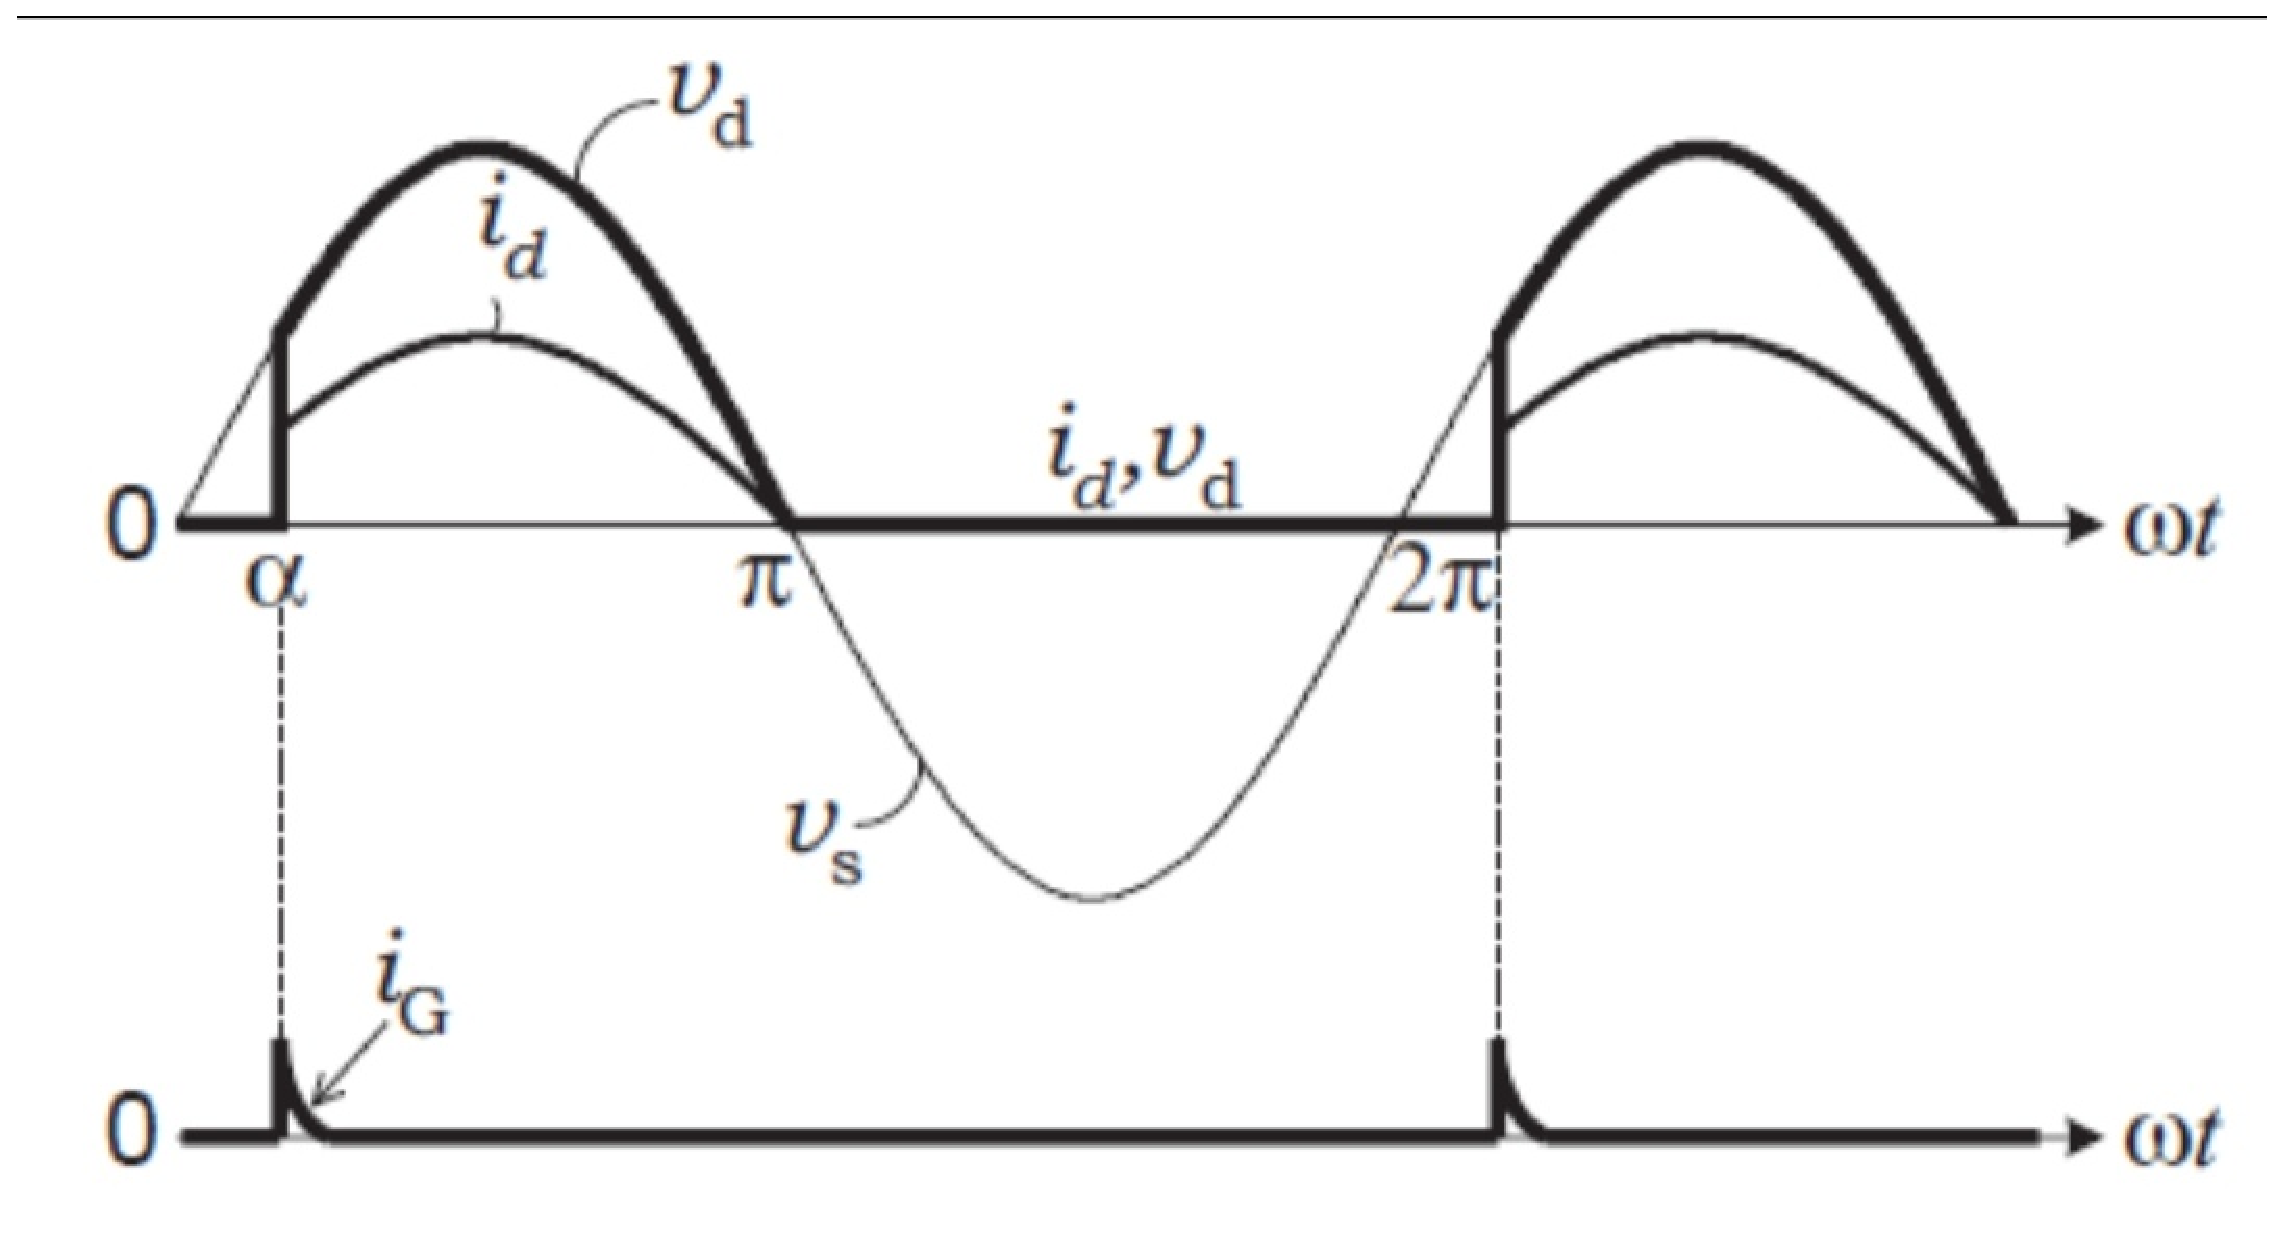
\includegraphics[width=\columnwidth]{./figs/fig2.eps}

\caption{Transistor Analogy} 
\label{fig2}
\end{figure}


\section{Working}
In single-phase half-wave rectifier, only one thyristor is used to control the load voltage. The thyristor will conduct (ON state) when the voltage $V_t$ is positive ($V_t > 0$) and a firing current pulse $I_g$ is applied to the gate terminal. Delaying the firing pulse by an angle ‘$\alpha$’ does the control of the load voltage. In the figure below the angle ‘$\alpha$’ is measured from the zero crossing point of the supply voltage $V_s$ .\\
The load is resistive and therefore current $i_d$ has the same waveform as the load voltage. The thyristor goes to the non-conducting condition (OFF state) when the load voltage and, consequently, the current try to reach a negative value.



 \section{Connections}
\begin{enumerate}
\item 
All grounded terminals are connected together.\item  In the circuit there are two optocouplers, optocoupler-1 to detect the zero crossing of the AC voltage signal and optocoupler-2 for firing the SCR. 
\item The optocouplers are used to isolate the Arduino (control circuit) from the power circuit.
\item  Diodes D1 and D2 are with the same type (1N4007), D1 is used to protect optocoupler-1 from reverse voltage and D2 to feed the SCR gate with positive current.
\item Optocoupler-1 collector pin is connected to Arduino pin 2 which is external interrupt pin, so optocoupler-1 interrupts the Arduino when there is a zero crossing event(when the AC signal goes from positive to negative).
\item When the AC voltage is positive, optocoupler-1 is ON and therefore the collector pin is connected to ground.
\item Here we used the 10k$\ohm$ resistor as pull-up resistor for Arduino pin 2 because we’ve an open collector output (optocoupler-1).
\item The 10k ohm potentiometer is used to control firing angle.
\item 
We got the 12V AC (50Hz) using a step down transformer (220V to 12V).

\end{enumerate}


\section{Calculation}
 Let, the input voltage $v_i$ be a sinusoidal voltage of amplitude Vm and frequency f Hz and let be given by,\\
% \begin{equation}
 \begin{equation}
 V_i=V_m \sin{\omega t}= V_m \sin{\theta}
 \end{equation}
%\end{equation}  
% V_{i= V_{m}$\sin{\omega}{t}$= V_{m}$\sin{\theta}$
Where $\omega$ is the angular frequency in radians/second and equals 2 $\pi f$.

Let, $\alpha$ be the firing angle i.e. the angle at which conducting begins. The SCR conducts from $\alpha$ to $\pi$ radians during the positive half cycle and does not conduct during the negative half cycle.\\

Then the average output voltage $V_{av}$ is given by,\\

Eqn. \ref{int}shows integration
\begin{equation}
V_{av}=\frac{1}{2\pi}\int_{\alpha}^{pi}V_{m}\sin{\theta}d\theta
\label{int}
%\begin{align*}
=\frac{V_m}{2\pi} (1+\cos{\alpha})
%\end{align*}
\end{equation}
Average current is given by:-
\begin{equation}
%\begin{align*}
I_{av}=\frac{V_{av}}{RL}=\frac{V_{m}}{2{\pi}RL}(1+\cos{\alpha})
%\end{align*}
\end{equation}

Thus as $\alpha$ increases from 0 to $\dfrac{\pi}{2}$ radians, (1 + $\cos \alpha$) reduces and $I_{av}$ reduces. Hence, by varying resistor R. we may control the gate current, control the firing angle and hence control $V_{av}$ and $I_{av}$.\\


\problem
Program the Arduino to generate the output voltage and the zero crossing detector to know the function of SCR.


\begin{figure}[t!]
\centering
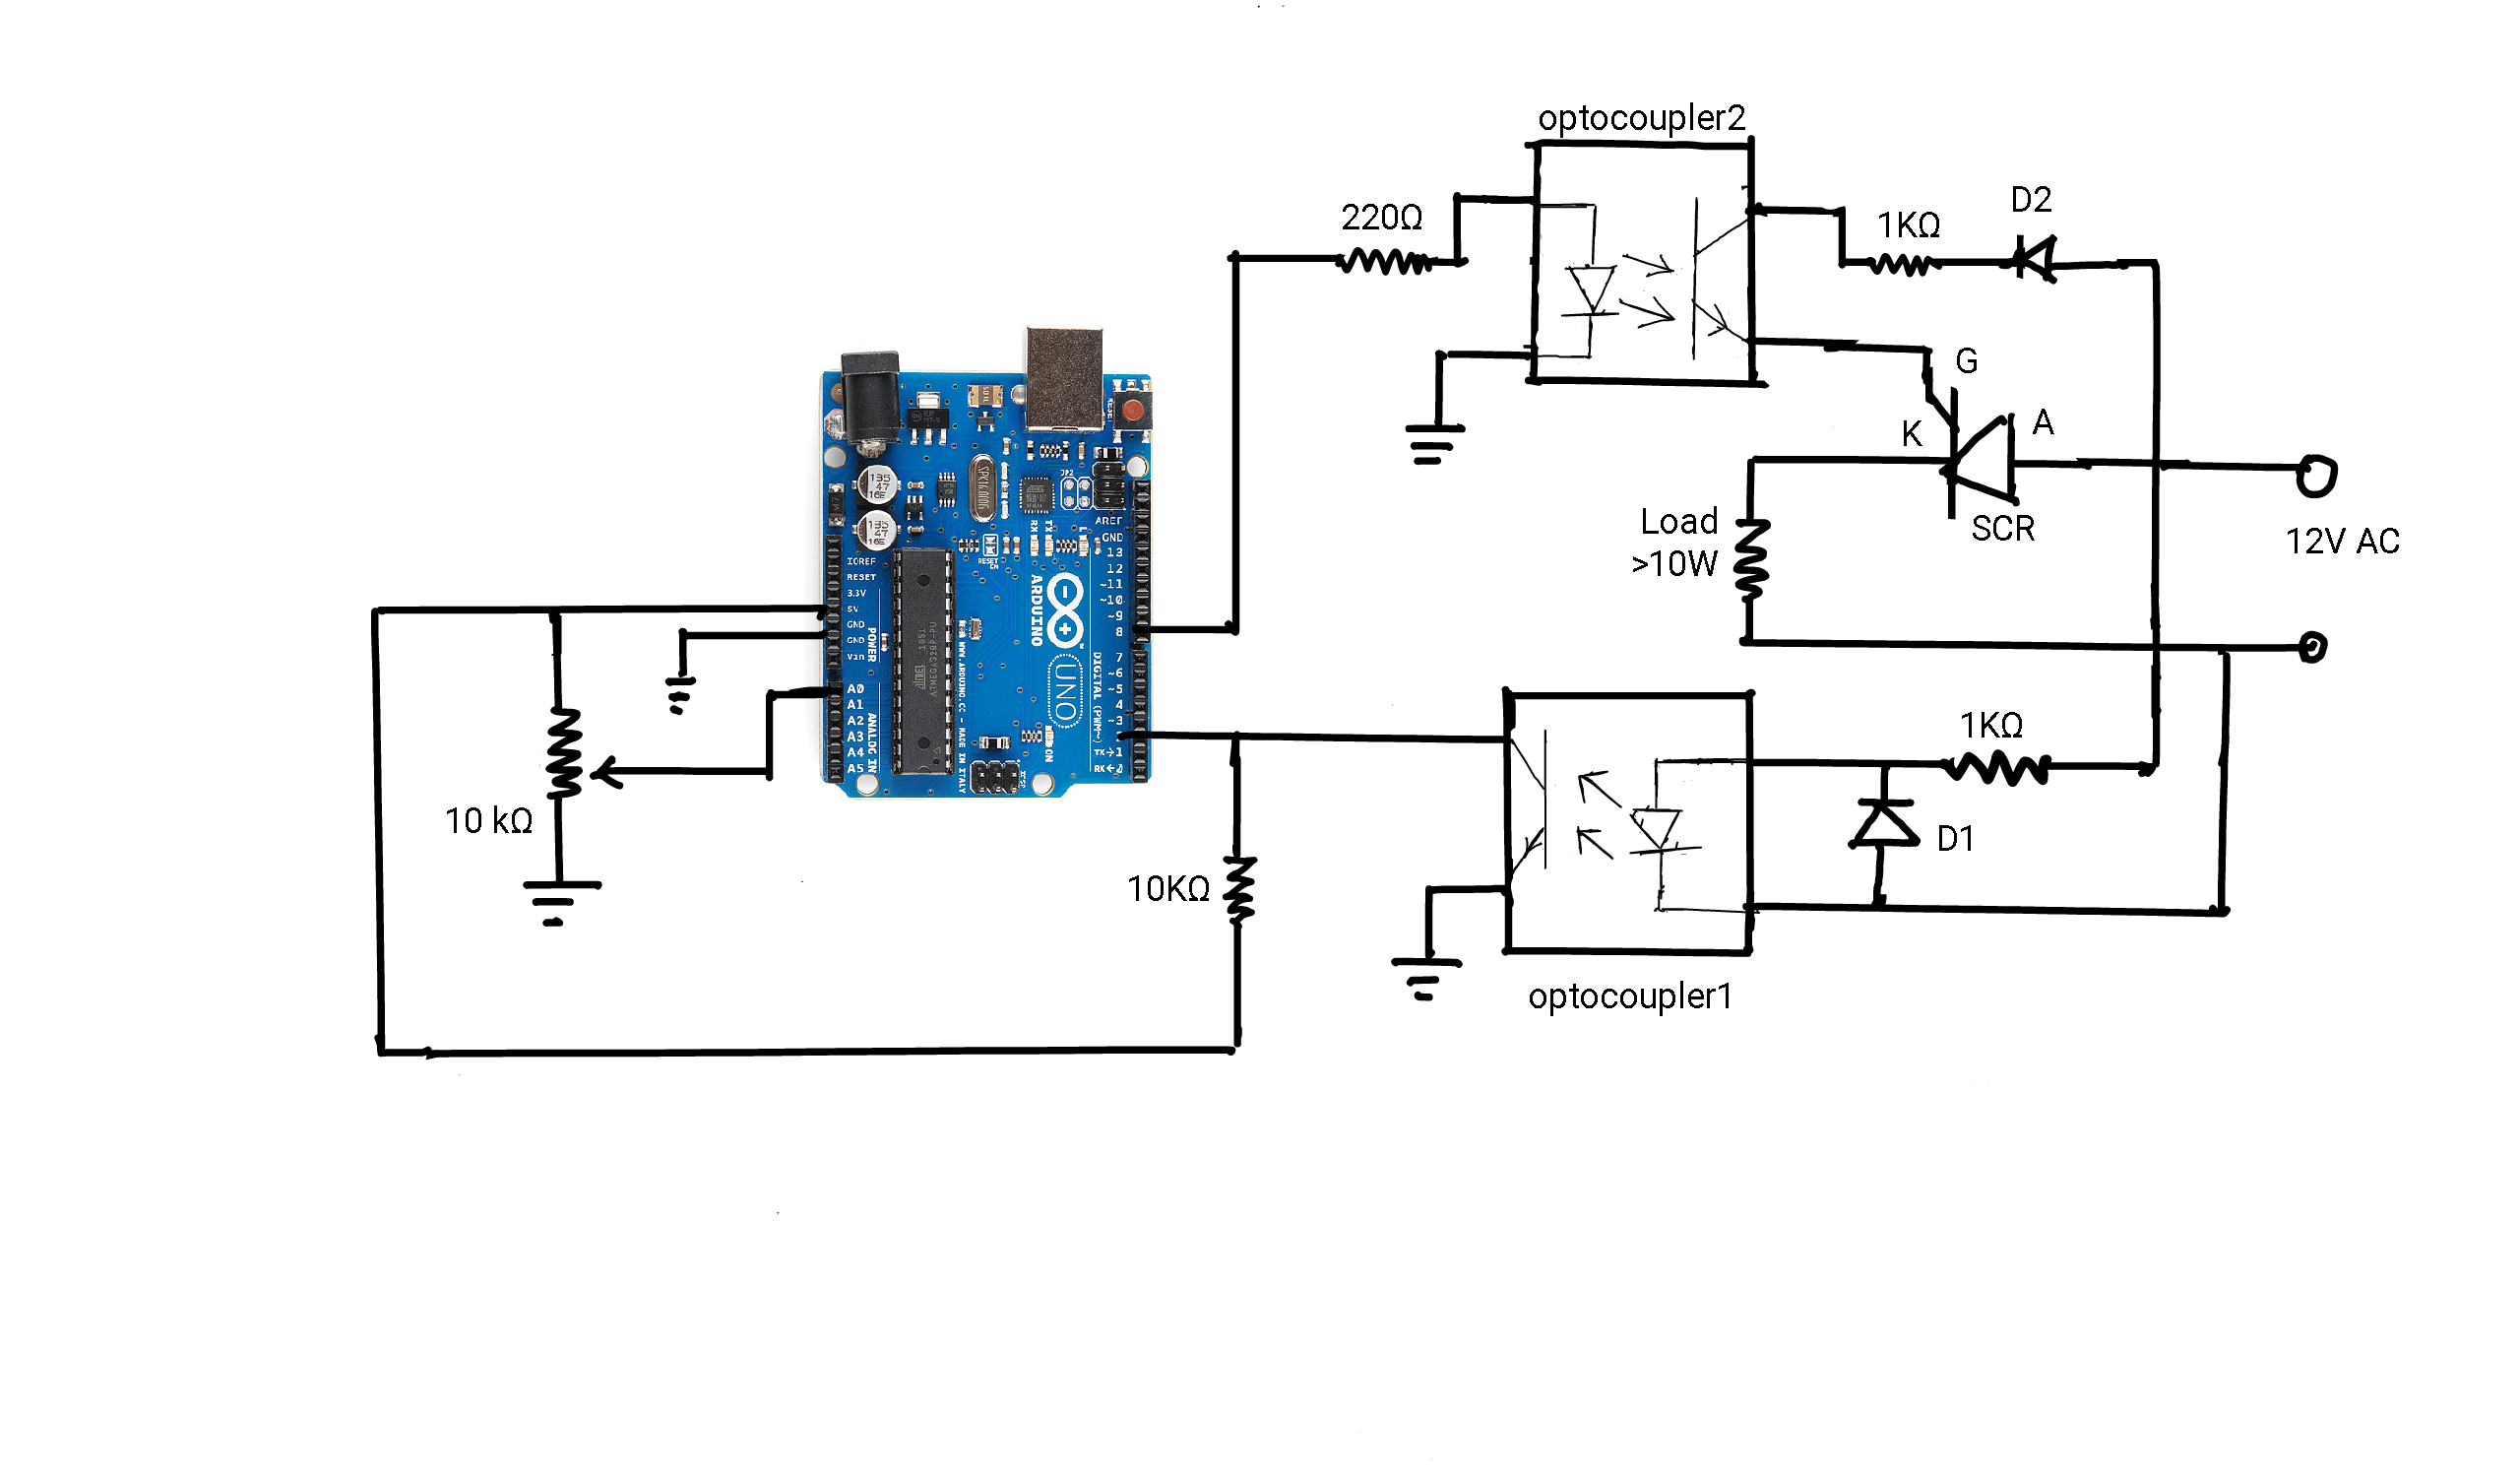
\includegraphics[width=20.0cm]{./figs/thumbnail.eps}

\caption{Circuit Operation  } 
\label{fig3}
\end{figure}

\end{document}
